\section{Firmware und FPGA-Code}

Der Zynq Ultrascale+ SoC hat ein ARM-Prozessorsystem und ein FPGA-System auf einem Chip. Gebootet wird immer zuerst das ARM-System, welches dann den FPGA konfiguriert. Der Code für das Prozessorsystem nennen wir Firmware und liegt nach dem Bootvorgang auf dem RAM, von wo die Prozessoren auf die Daten und Instruktionen zugreifen. Der FPGA wird mit dem Bitfile geladen, welches den implementierten Code für den FPGA enthält. 

\begin{figure}[tb]
    \centering
    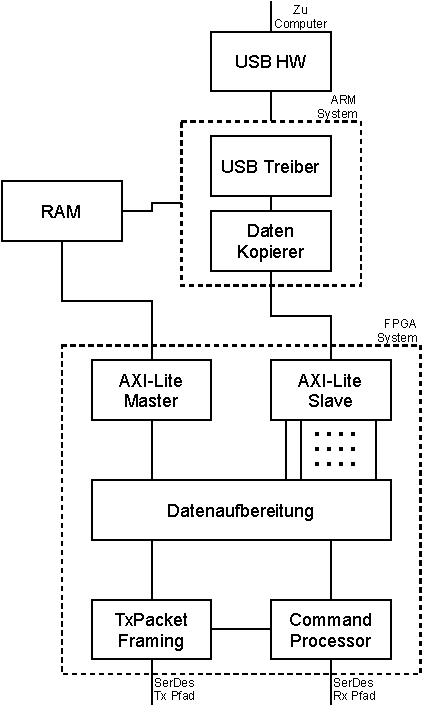
\includegraphics[width=0.5\linewidth]{bd_firmware}
    \caption{Blockdiagramm der Firmware und FPGA-Codes}
    \label{fig:bd_firmware}
\end{figure}

Abbildung \ref{fig:bd_firmware} enthält das Blockdiagramm vom Aufbau der Firmware und des FPGA-Codes. Vom Prozessorsystem wird nur der ARM Cortex-R5 verwendet. Dafür gibt es die folgenden zwei Gründe:

\begin{enumerate}
    \item Der Cortex-R ist weniger komplex als der Cortex-A Kern. Der grösste Unterschied zwischen dem R- und dem A-Kern ist die Memory Management Unit (MMU). Der ARM Cortex-A besitzt eine MMU, welcher den Speicher virtualisiert und den den Zugriff auf jenen Überwacht. Der ARM Cortex-R Kern besitzt nur eine Memory Protection Unit (PMU). Diese virtualisiert den Adressraum nicht, sondern arbeiten mit den physikalischen Adressen. Die PMU überwacht jedoch auch den Zugriff auf den Speicher. Da die Virtualisierung des Adressraums nicht benötigt wird, kann diese Komplexität somit gespart werden. 
    \item Der Cortex-R liegt in der Low Power Domain und der Cortex-A in der High Power Domain. Diese beiden Domänen können separat gespeist werden. Dies erlaubt A-Kerne auszuschalten und vom Stromkreis zu trennen. Somit reduziert sich der Energieverbrauch des SoCs und auch die produzierte Wärme, welche über das Gehäuse dis­si­pie­rt wird.
\end{enumerate}

Der Computer kann über USB die Bilder und die Konfiguration auf das RAM laden. Der \textit{USB Treiber} schreibt diese direkt auf das RAM und benachrichtigt die \textit{Daten Kopier} Funktion, dass neue Konfigurationen vorhanden sind. Auf die Bilder kann der FPGA über eine AXI-Schnittstelle zugreifen mittels dem \textit{AXI-Lite Master} Modul. Die Konfigurationen werden vom ARM direkt auf Register im FPGA geschrieben. Dies passiert auch über eine AXI-Schnittstelle. Die Konfiguration werden sofort in die FPGA-Register geschrieben, damit der FPGA auf alle Konfigurationen parallel zugreifen kann und diese nicht andauernd abfragen muss. Dies übernimmt das \textit{AXI-Lite Slave} Modul.

FPGA-Blöcke \textit{TxPacketFraming} und \textit{CommandProcessor} sind Blöcke, welche wir von dem System der Varian übernehmen können. Jedoch emulieren diese Blöcke die Startup-Sequenz des Sensors nicht. Somit müssen sie noch für unser System angepasst werden. Das \textit{CommandProcessor} Modul empfängt die Befehle des XI-Computers und gibt die Write- und Trigger-Befehle weiter. Die Read-Befehle gibt es direkt an das \textit{TxPacketFraming} Modul weiter. 
%Das \textit{Access Control} Modul speichert die Write-Befehle und gibt Zugriff auf die gespeicherten Konfigurationen und initiiert die Trigger-Befehle. 
Das \textit{Tx Packet Framing} Modul sendet die Daten an den XI-Computer.

Die \textit{Datenaufbereitung} bearbeitet die Bilder mit Pixelfehlern, koordiniert das Senden der Bilder und Arbeitet die Befehle des XI-Computers ab. Dieser Block ist noch nicht Teil von diesem Projekt und wird im nächsten Semester in der weiterführenden Bachelorthesis implementiert.

So soll es auf dem endgültigen System aufgebaut sein. Auf dem PE1-Board, also dem Zwischensystem, ist es wie in Abbildung \ref{fig:bd_firmware_pe1}. Da der externe SerDes und das SFP-Modul noch nicht vorhanden sind, sind die Blöcke der Varian nicht implementiert. Das Zwischensystem zeigt, dass der PC über USB Daten auf das RAM schreiben kann, dass der ARM-Kern diese Daten über AXI in Register im FPGA schreiben kann, und dass der FPGA über AXI auf das RAM zugegriffen kann. Um dies zu zeigen, ist das Register, auf welches der ARM-Kern schreibt, mit einem LED verbunden und das \textit{AXI-Lite Master} Modul mit zwei LEDs, welche anzeigen, ob der Schreib- und Lesezyklus fertig ist und ob er erfolgreich war. Zudem gibt der ARM-Kern über UART den Wert des RAM-Registers und des FPGA-Registers aus. Über einen DIP-Switch kann man den Wert einstellen, welcher das FPGA in das RAM schreiben soll. 

\begin{figure}[tb]
    \centering
    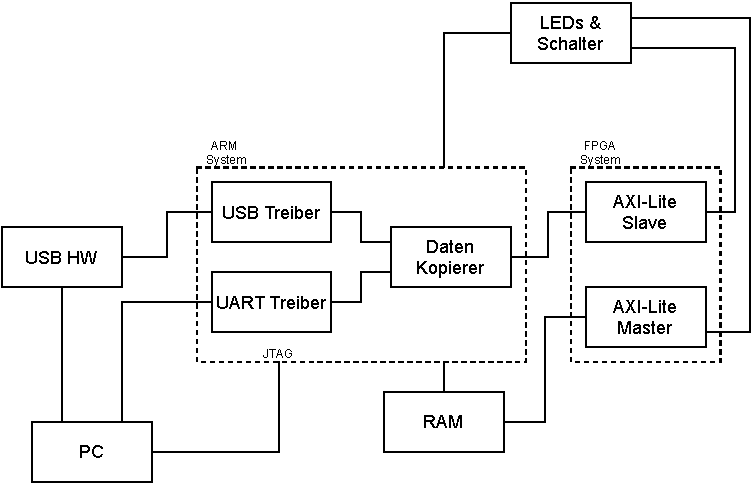
\includegraphics[width=\linewidth]{bd_firmware_pe1}
    \caption{Blockdiagramm der Firmware und FPGA-Codes auf dem Entwicklungssystem}
    \label{fig:bd_firmware_pe1}
\end{figure}

\subsection{ARM Firmware}
Die Firmware für den ARM Cortex R5 besteht aus vier Teilen. Dem \textit{USB-Treiber}, der \textit{Daten Kopierer} Funktion, dem \textit{IO-Treiber} und der \textit{Main} Funktion. Den \textit{USB-Treiber} haben wir von Xilinx übernommen und ein wenig angepasst. Der \textit{Daten Kopierer} hat eine Struktur, welche die Konfigurationen auf die Register in FPGA schreibt, sobald der \textit{USB-Treiber} meldet, dass die Konfigurationen geändert wurden. Über den \textit{IO-Treiber} kann man die LEDs, Taster und Schalter ein- und auslesen, ohne sich Gedanken über die physikalische Anordnung der IOs zu machen. Die \textit{Main} Funktion verbindet die Blöcke und gibt für Testzwecke Informationen über UART oder die LEDs weiter.

\subsubsection*{USB-Treiber}
Der \textit{USB-Treiber} ist das grösste Modul der ARM-Firmware. Daher wird diese ein wenig genauer beschrieben. Leider hat sich Xilinx nicht viel Aufwand für das Konzept, die Lesbarkeit und die Dokumentation des USB-Treibers gemacht.

Der \textit{USB-Treiber} verwendet zum einen den USB-Treiber, welcher im Board Support Package (BSP) im Platform Projekt von Vitis vorhanden ist. Und zum anderen das Beispiel Projekt, welches Xilinx mit dem Treiber mitliefert. Der USB-Treiber des BSPs hat Funktionen und Datenstrukuren, um die Grundlegenden Funktionen des USB-Moduls zu steuern. Das Beispielprojekt implementiert den Softwareteil des USB-Standards und der Massstorage USB-Klasse. Das Beispielprojekt unterstützt den reduzierten SCSI Befehlssatz, um die Massstorage Klasse zu implementieren.

Das Beispielprojekt greift auf die Funktionen des USB-Treibers des BSPs über eine Wrapper-Library zu. Diese Bibliothek ändert die API des USB-Treibers des BSPs. Jedoch greift das Beispielprojekt trotzdem noch direkt auf den USB-Treiber des BSPs zu. 

Am Beispielprojekt wurde nicht viel geändert. Zum einen wurde in der Datei \textit{xusb\_class\_\-storage.c} hineingefügt, dass wenn in Sector Eins geschrieben wird, dass das Flag \textit{configWrite} gesetzt wird. Somit wird der Daten Kopier Funktion mitgeteilt, das neue Konfigurationsdaten vorhanden sind. Die grösse des Speichers, die der USB-Treiber als Massenspeicher hat kann in der H-Datei \textit{xusb\_class\_storage.h} unter VFLASH\_SIZE eingestellt werden. Im Moment ist es auf 1.5GB eingestellt.
Die USB Strukturen, welche dem Host mitteilen, was das USB Device für ein Gerät ist sind unter \textit{xusb\_ch9\_storage.ch} zu finden.

\subsection{AXI FPGA-Module}
\label{sec:axi}
Die AXI FPGA-Module sind Vorlagen von Xilinx. Der AXI-Lite Slave nimmt Daten über das AXI Protokoll entgegen, speichert diese in Registern im FPGA und gibt die Daten wieder aus, wenn ein entsprechender AXI-Befehl ankommt. Der AXI-Lite Master schreibt sequenziell über AXI auf eine Reihe von Registern und liest diese anschliessend wieder aus und vergleicht sie mit den geschriebenen Werten. Beide Module implementiereren die AXI-Protokolle, indem sie für jeden Ausgang einen VHDL-Prozess definieren, welcher den Wert des Ausgangs anhand von den Eingängen bestimmt. Wenn die Eingänge zu wenig Information geben um die Zustände des Ausgangs komplet zu beschreiben, führen sie noch Zwischensignale ein.


\subsection{Varian FPGA-Module}
Die beiden Module \textit{TxPacketFraming} und \textit{CommandProcessor} sind von der Firma Varian geschrieben. Für dieses Projekt können wir sie grössten Teils übernehmen. Abbildung \ref{fig:bd_fpga_varian} zeigt das Blockschaltbild der beiden Module und wie sie zusammengehängt sind.

\begin{figure}[tb]
    \centering
    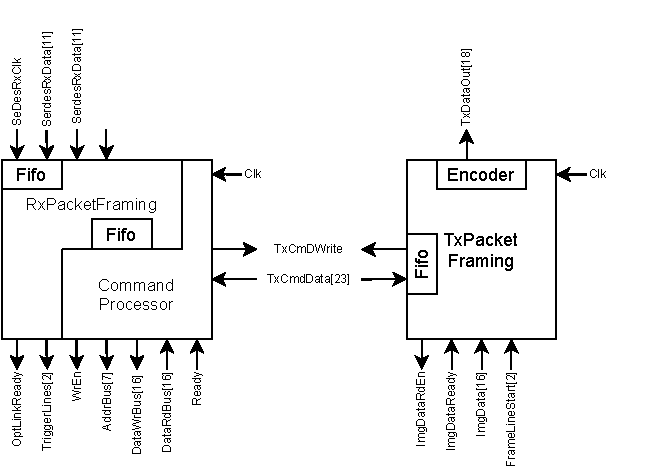
\includegraphics[width=\linewidth]{bd_fpga_varian}
    \caption{Blockdiagramm der beiden Module \textit{TxPacketFraming} und \textit{TxPacketFraming}}
    \label{fig:bd_fpga_varian}
\end{figure}

\subsubsection*{TxPacketFraming}
Das Modul \textit{TxPacketFraming} ist zuständig für die Übertragung der Daten an den XI-Computer über den externen SerDes. Da der externe SerDes eine DC-freie codierung besitzt, muss dies im FPGA geschehen. Dafür werden die Daten zuerst vom \textit{Encoder} Modul kodiert, bevor sie an den SerDes gesendet werden. Das \textit{Encoder} Modul hat vier Eingänge und einen Ausgang.
Der \textbf{Clk}-Eingang ist der Takt des Moduls.
Der \textbf{Code}-Eingang zeigt, ob es sich um ein Signal oder um Bilddaten handelt.
Der \textbf{En}-Eingang aktiviert das Modul.
Im \textbf{DataIn}-Eingang werden die Daten und Signale eingegeben.
Der \textbf{DataOut} Ausgang gibt die codierten Daten und Signale aus.

Der Imager sendet entweder Bilddaten oder Antworten von Befehlen des XI-Computers. Vor jedem neuen Bild sendet der Imager ein \textit{Frame Start} Signal, vor jeder neuen Zeile eines Bildes eine \textit{Line Start} Signal und vor jeder Antwort eines Befehls ein \textit{Command} Signal. Wie in Kapitel \ref{sec:varian_com} unter \textit{Kommunikation zwischen Imager und XI-Computer} erläutert.

Der Tx-Pfad des SerDes hat 18 parallele Bits. 16 werden gebraucht, um die Daten und Signale zu übertragen, eines um zu signalisieren, ob es sich um ein Signal oder um Daten handelt und das letzte, um das DC-Balancing zu implementieren.

Die Antworten auf einen Read-Befehl werden vom \textit{CommandProcessor} mit den Eingängen \textbf{TxCmdWrite} und \textbf{TxCmdData} in ein Fifo geschrieben und bei Gelegenheit, zwischen den Bildzeilen, übertragen.
Um eine Bildzeile zu übertragen muss der Eingang \textbf{ImgDataReady} gesetzt werden und den \textbf{FrameLineStart}-Eingang entsprechend gesetzt werden. Für ein neues Bild muss \textit{0b10} und für eine neue Zeile \textit{0b01} angelegt werden. Wenn das \textit{TxPacketFraming} Modul bereit ist die Zeile zu übertragen bestätigt es dies mit dem Setzen des Ausgangs \textbf{ImgDataRdEn}. Im nächsten Takt überträgt das Modul das Signal und danach überträgt es pro Takt einen Pixel. Dafür müssen die Pixeldaten am Eingang {ImgData} angelegt werden und mit jedem Takt entsprechend dem nächsten Pixel erneuert werden. Sobald alle Pixel der Zeile übertragen sind muss der \textbf{ImgDataReady}-Eingang gelöscht werden. Am \textbf{Clk}-Eingang muss der Takt angelegt werden und der Ausgang \textbf{TxDataOut} geht auf die Pins, welche mit dem Externen SerDes verbunden sind.

Dieses Verhalten ist mittels einer Finite State Machine (FSM) gelöst. Die FSM ist in Abbildung \ref{fig:fsm_tx_packet_framing} zu sehen.

\begin{figure}[H]
    \centering
    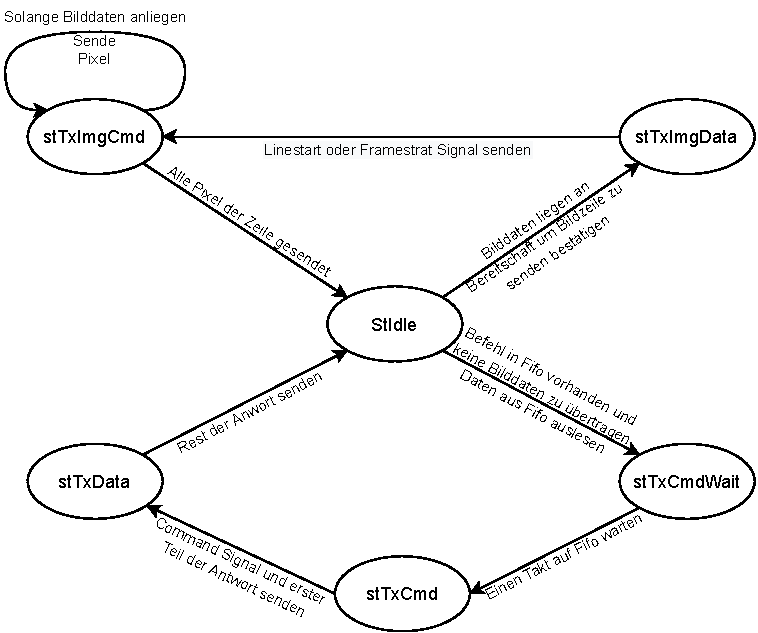
\includegraphics[width=0.8\linewidth]{fsm_tx_packet_framing}
    \caption{State Machine des Moduls \textit{TxPacketFraming}}
    \label{fig:fsm_tx_packet_framing}
\end{figure}

\subsubsection*{CommandProcessor}
Das Modul \textit{CommandProcessor} beinhaltet das Modul \textit{RxPacketframing}. Dieses beinhaltet wiederum zwei Fifos. Eines direkt am Rx-Eingang vom SerDes, welches zwischen dem FPGA-Takt und dem SerDes-Takt wechselt. Und ein weiteres um die Daten für den \textit{CommandProcessor} bereit zu stellen. Das erste Fifo ist nur aktiv, wenn das SFP und der SerDes parat sind. Dafür sind die Eingänge \textbf{nSerdesLock} und \textbf{OptoSD}. Zudem wird eine UND-Verküpfung der beiden Signale am Ausgang \textbf{OptlinkReady} ausgegeben. Das Modul \textit{RxPacketframing} unterscheidet zwischen den drei verschiedenen Befehlen des XI-Computers. Ein Trigger-Befehl gibt es direkt an den Ausgang \textbf{Triggerlines}. Und die Read- und Write-Befehle schreibt es in das zweite Fifo. Wenn das erste Bit eine "0" ist, handelt es sich um einen Read-Befehl und ansonsten um einen Write-Befehl. Die nächsten sechs Bits im Fifo geben die Adresse de Read- oder Write-Zugriffs an. Und die zwei Byte sind nur für den Write-Befehl relevant und enthalten die zu schreibenden Daten. Dieses Verhalten ist in der FSM in Abbildung \ref{fig:fsm_rx_packet_framing} zu sehen.

\begin{figure}[H]
    \centering
    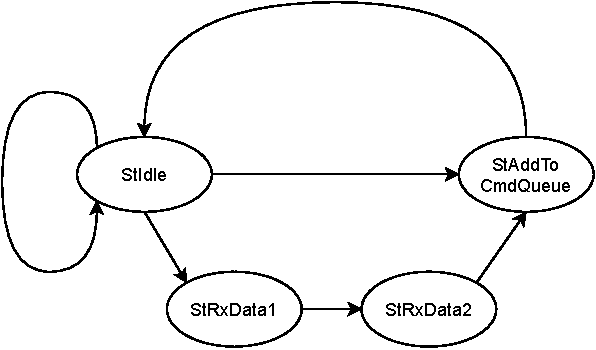
\includegraphics[width=0.6\linewidth]{fsm_rx_packet_framing}
    \caption{State Machine des Moduls \textit{RxPacketFraming}}
    \label{fig:fsm_rx_packet_framing}
\end{figure}

Der \textit{CommandProcessor} nimmt die Daten aus dem Fifo und arbeitet diese ab. Wenn es sich um einen Write-Befehl handelt, sendet er die Daten zu den Einstellungsregistern. Wenn es sich um einen Read-Befehl handelt liest er die Daten von den Einstellungsregistern und gibt die Daten über die Ausgänge \textbf{TxCmdWrite} und \textbf{TxCmdData} an das Fifo des Moduls \textit{TxPacketFraming} weiter.

Die Schnittstelle zu den Einstellungsregistern besteht aus den Ausgängen \textbf{WrEn}, \textbf{AddrBus}, \textbf{DataWrBus} und aus den Eingängen \textbf{DataRdBus}, \textbf{Ready}.
Wenn der Ausgang \textbf{WrEn} gesetzt ist, handelt es sich um einen Write-Zugriff und ansonsten um einen Read-Zugriff. Sobald der Eingang \textbf{Ready} gesetzt wird, heisst es, dass der Zugriff erfolgreich war. Der \textbf{Ready} Eingang wird erst ein Takt nach dem Anlegen der Adresse und der Daten geprüft. Die Adresse wird am Ausgang \textbf{AddrBus} angelegt, die zu schreibenden Daten an dem \textbf{DataWrBus} und die zu lesenden Daten werden vom Eingang \textbf{DataRdBus} gelesen. Dieses Verhalten ist mit der FSM in Abbildung \ref{fig:fsm_command_processor} implementiert.

\begin{figure}[tb]
    \centering
    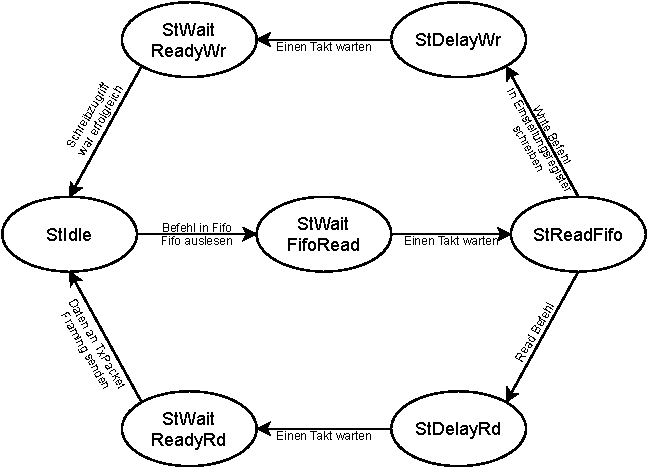
\includegraphics[width=\linewidth]{fsm_command_processor}
    \caption{State Machine des Moduls \textit{CommandProcessor}}
    \label{fig:fsm_command_processor}
\end{figure}

\subsection{Vivado Projekt}
Das Vivado Projekt kann mit dem Skript erstellt werden. Das Skript kreiert ein neues Projekt, erstellt ein Blockdiagramm im IP Integrator, fügt alle Blöcke in das Blockdiagramm, konfiguriert das Prozessorsystem im Blockdiagramm, erstellt die Top- und die Constraint-Dateien.

Die Top-Datei instantiiert das Blockdiagramm vom IP Integrator und definiert die Namen der Ausgänge, welche an die Pins gehen. Die Constraint-Datei verbindet die Ausgänge der Top-Datei mit den Pins und konfiguriert die Pins entsprechend. 

Im Skript muss der Pfad, wo das Skript liegt aktualisiert werden. Das Skript erstellt anschliessend das Projekt in einem Unterordner, welches wie das Projekt heisst. Die Source-Dateien müssen in einem Unterordner namens \textit{src} liegen.

Das Skript kann mit dem Befehl \textit{source \{Skriptpfad/Skriptname\}} in der TCL-Console in Vivado gestartet werden. Wobei der Skriptpfad und Skriptname dementsprechend ersetzt werden müssen.

\subsection{Vitis Projekt}
Das Vitis Projekt kann auch mit einem Skript erstellt werden. Es gibt zwei Skripte. In beiden muss der Pfad in dem das Skript liegt aktualisiert werden. Die exportierte XSA-Datei muss im gleichen Ordner wie das Skript sein und top.xsa heissen. Zudem braucht es noch einen Ordner namens "Vitis", in welchem Vitis gestartet werden muss, worin danach die XSCT-Console gestartet werden kann. Das erst Skript erstellt die ELF-Dateien für den FSBL und die PMU-Firmware und fügt diese mit dem ELF-File der Applikation und dem Bitstream zu einem bootbaren Image zusammen. Die ELF-Datei der Applikation muss auch im selben Ordner sein, wie das Skript.

Das zweite Skript erstellt ein Projekt in Vitis mit der Plattform, dem System und der Applikation. Es compiliert das Plattform-Projekt und importiert die Source-Dateien vom Unterordner "src" in das Applikations-Projekt.  

Das Skript kann mit dem Befehl \textit{source \{Skriptpfad/Skriptname\}} in der XSCT-Console in Vitis gstartet werden. Wobei der Skriptpfad und Skriptname dementsprechend ersetzt werden müssen.

